\subsection{Quadratic function}
Lets consider a simple 2D quadratic function given by:
\begin{align}
	f(\bm{x}) = \frac{1}{2D}\left( x_1^2 + x_2^2\right)
\end{align}
with $\bm{x} = (x_1,x_2)$. For the function, consider the problem:
\be
\min_{\bs{x}} f(\bs{x}), \qquad \textrm{ such that $x_1 \geq 1$ }
\ee
%
Following from Eq.\ref{eq:U_theta_constraint}, the upper bound can be given by the following for a Gaussian with the variational parameter $\theta$:
\begin{align}
	U(\bm{\theta}) = \E_{\bm{x}\sim \mathcal{N}(\bm{x}\mid \bm{\theta})}\left[ f(\bm{x}) + \max (1-x_1,0)\right]
\end{align}
with $\bm{\theta} = (\mu,\sigma)$. The gradients of the upper bound $U(\bm{\theta})$ can be approximated as discussed in Eq. \ref{eq:VO_grad_estimator} using Monte Carlo. With the learning rate $\eta=0.1$, initial noise $\sigma = 5$ and ADAM optimizer to perform the optimization, we obtain the results discussed in Figure \ref{fig:VO}. Figure \ref{fig:VO_no_cons} discusses the results when the constraints are not considered and Figure \ref{fig:VO_constraints} discusses the results with the constraints. As we can see from the figures that the noisy gradient estimates are able to drive that optimizer to the minimum. Especially in the case of Figure \ref{fig:VO_constraints}, two different starting point are studied. One which starts in a domain where the constraints are met (in red) and the next where the constraints are violated (in yellow). In both the cases, the optimizer moves towards the minimum while satisfying the constraints, thus converging close to $(x_1,x_2)= (1,0)$. Its also noteworthy to observe that the variance $\sigma^2$ reduces as we near the minimum.  

\begin{figure}[!htpb]
	\centering
	\begin{subfigure}{0.75\textwidth}
		\centering
		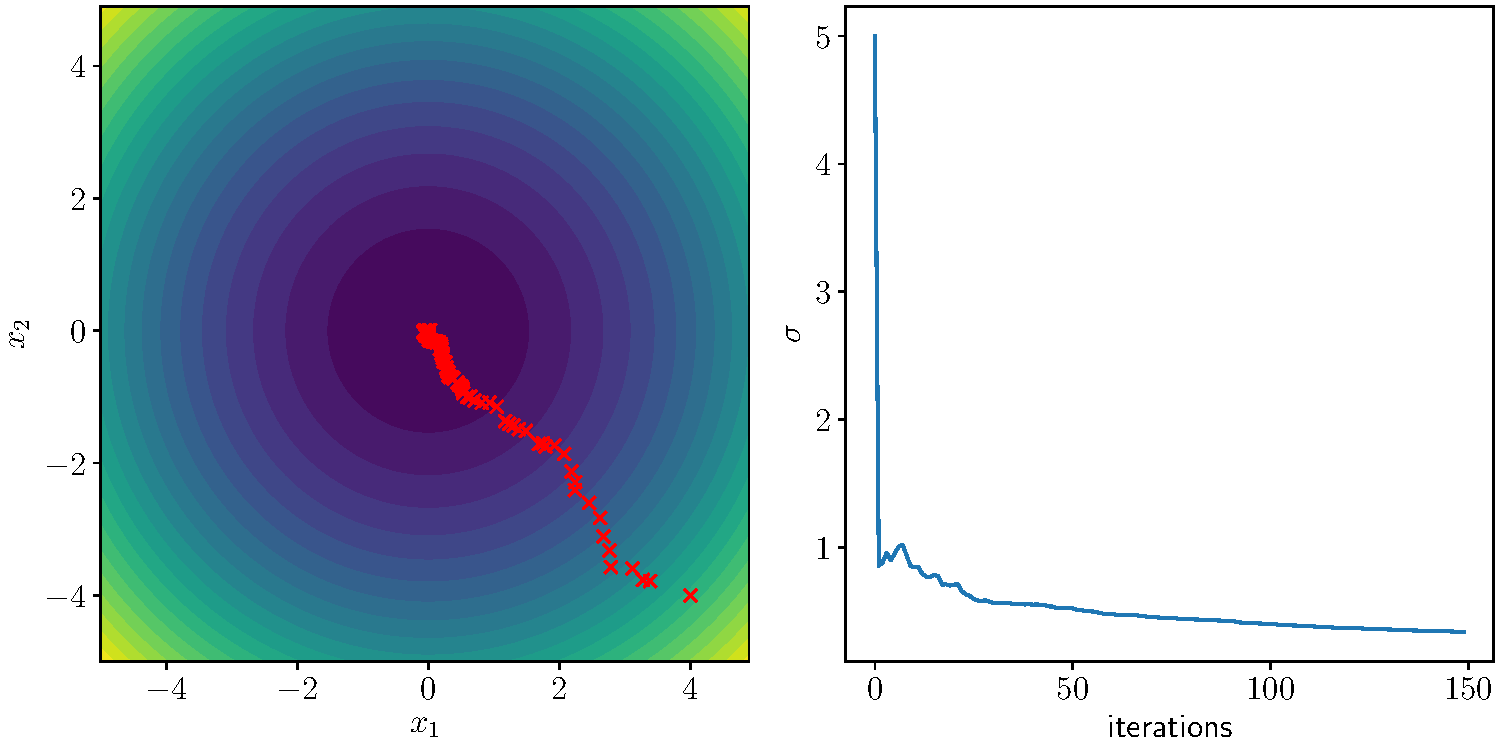
\includegraphics[width=\linewidth]{../figures/TUM/theta_evolution_VO_2023_02_21-03_34_28_PM.pdf}
		\caption{}
		\label{fig:VO_no_cons}
	\end{subfigure}
	\begin{subfigure}{0.75\textwidth}
		\centering
		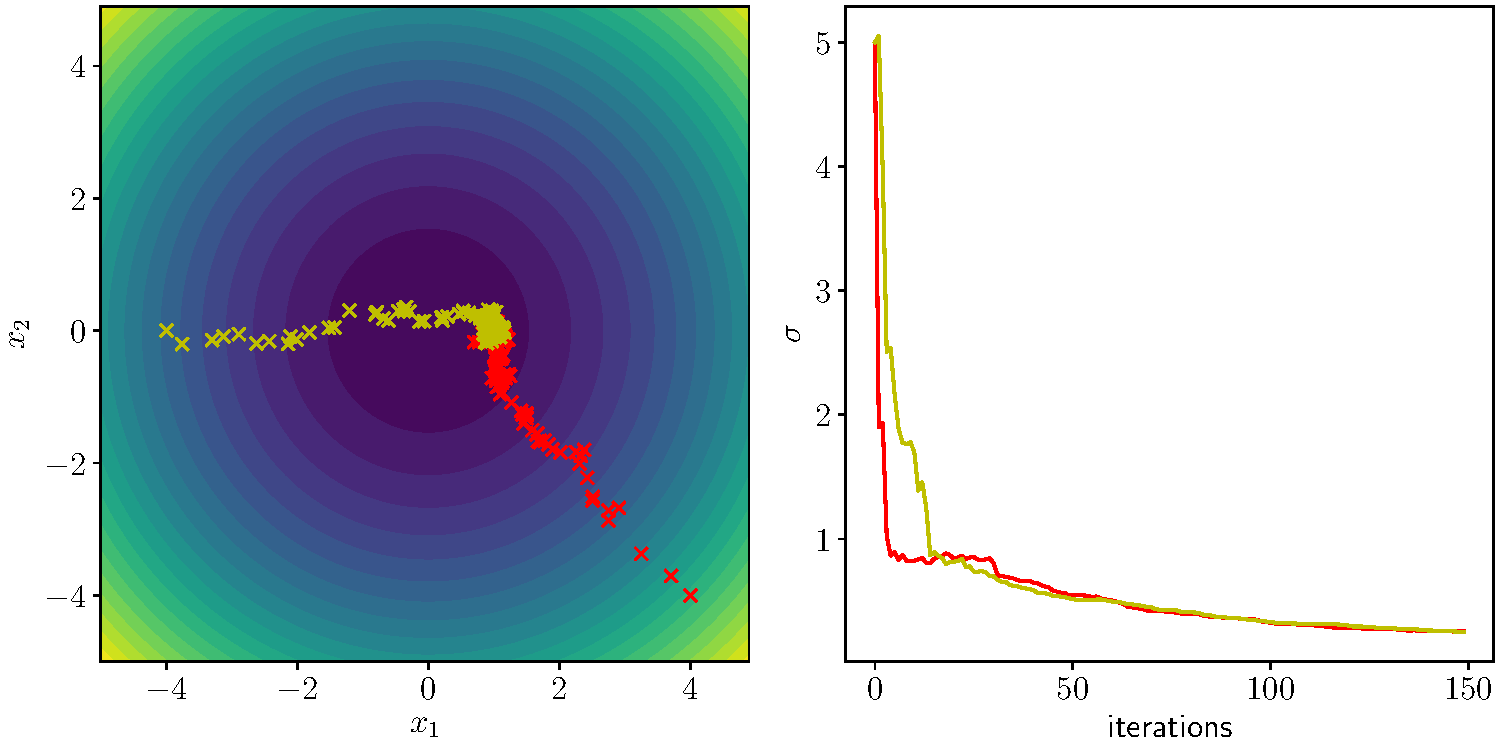
\includegraphics[width=\linewidth]{../figures/TUM/theta_evolution_VO_constraints_2023_02_24-05_12_07_PM.pdf}
		\caption{}
		\label{fig:VO_constraints}
	\end{subfigure}
	\caption{\emph{Stochastic VO for constrained and unconstrained quadratic function}: (a) This is for case when constraints are not present. The left plot shows how the Gaussian mean $\mu$ move towards the minimum of objective despite noisy gradients, the right plots the learned $\sigma$ values versus the gradient descent iterations (b) This is for a constraint on $\bm{x} (x_1 \geq 1)$. The left plot shows how the Gaussian mean $\mu$ moves towards the optimum (for two different starting values) while trying to satisfy the constraint and the right plots the learned $\sigma$ values versus the gradient descent iterations   }
	\label{fig:VO}
\end{figure}

\begin{mdframed}
	\textbf{Open research question/Novelty :} 
	\begin{enumerate}
		\item Why not use finite differences to approximate gradients?: With the constraints, the augmented objective is $C^0$, so the gradients are not even defined at that point.
		\item Then why not use Bayesian Optimization? \atul{Bayesian optimization is difficult for $(dim \geq 10)$. Also constraints are "difficult" in Bayesian optimization. The VO most probably will also struggle in high dimention. Have to check. But including constraints is not that difficult. Stelios: For the current toy problem, BO may be better (because objective has no random variable). But for the problem when the objective has implicit dependance on the design variable (through a random variable), BO makes no sense. The objective would not be known}
		\item To test in high dimention, Will it make sense to test the VO with the following?:
		\begin{align}
			f(x) = \frac{1}{200}\sum_{i=1}^{100} x_i^2 \quad \text{s.t} \quad x_i\geq1
		\end{align}
		The $\bm{x}^*$ would be a unit vector.
	\end{enumerate}
\end{mdframed}


\subsection{Performance based concrete design}

\begin{figure}[!htpb]
	\centering
	\begin{tikzpicture}
		\node (theta) at (-1,-2) {$\theta$};
		\node (x_1) at (0,0) {$x_1$};
		\node (x_2) at (0,-2) [circle, draw, dotted] {$x_2$};
		\node (b_1) at (1,1) [circle, draw] {$\bm{b}_1$}; % can add fill=black!20
		\node (b_2) at (1,0) [circle, draw] {$\bm{b}_2$};
		\node (y_1) at (3,1) [rectangle, draw] {$y_1$};
		\node (y_2) at (3,0) [rectangle, draw] {$y_2$}; 
		\node (y_3) at (3,-1) [rectangle, draw] {$y_3$}; 
		\node (y_4) at (3,-2) [rectangle, draw] {$y_4$}; 
		\node (C_1) at (5,1) [rectangle, draw] {$\mathcal{C}_1\left(y_1(\cdot)\right)$}; 
		\node (C_2) at (5,0) [rectangle, draw] {$\mathcal{C}_2\left(y_2(\cdot)\right)$}; 
		\node (C_3) at (5,-1) [rectangle, draw] {$\mathcal{C}_3\left(y_3(\cdot)\right)$}; 
		\node (O) at (5,-2) [rectangle, draw] {$\mathcal{O}\left(y_4(\cdot)\right)$}; 
		
		\graph {
			%A [as=$\mathcal{A}$, shape = none, "$P(A)$"];
			%B [as=$B$, shape=rectangle ,"$P(B)$"];
			%C [as=$C$,fill=black!20 , "$P(C|A,B)$"];
			
			(x_1) -> {(b_1),(b_2),(y_4)};
			(b_1) -> {(y_1),(y_2),(y_3)};
			(b_2) -> {(y_1),(y_2),(y_3)};
			(y_1) -> (C_1);
			(y_2) -> (C_2);
			(y_3) -> (C_3);
			(y_4) -> (O);
			(theta) -> (x_2);
			(x_2) -> {(y_1),(y_2),(y_3),(y_4)};
			
		};
	\end{tikzpicture}
	\caption{\emph{Stochastic computational graph for the constraint optimization problem for the performance based concrete design:} The circle represents \textit{stochastic nodes}, rectangle the \textit{deterministic node} and no shape is for the \textit{input nodes} (design variables). The objective and the constraints are explicitly dependant on the design variable $x_2$ and they are not differentiable w.r.t it (Hence $x_2$ in dotted). So based on our discussions above, $x_2 \sim q(x_2\mid\theta)$. Several other deterministic nodes are present between the random variables $\bm{b}_1$,$\bm{b}_2$ and the KPIs $y_1, y_2, y_3, y_4$ but they are ignored for brevity.}
	\label{fig:stochastic graph demonstrator}
\end{figure}

The interconnected graph in Figure. \ref{label} can be represented in term of probabilistic graphs as discussed in Figure. \ref{fig:stochastic graph demonstrator}

\atul{This section will involve the calibration results and then the optimization results. The concrete model discussed in section 2 IMO should be in a form accessible to computational science community, with details elaborated in Appendix. Drawing from discussions in section 2, we can discuss the results here.}